\subsection{Background}
\begin{frame}{Research focus}

\textcolor{blue}{Aim}:
    To identify the effect of the RKB approach on collaborative concept mapping in a practical classroom
    % Does the RKB approach affect co-construction of knowledge with concept maps? 
    %If so, to what extent?


\begin{block}{Sub-research questions}
    \begin{enumerate}
        \item <1-> Whether or not students are able to produce high quality group products? If so, to what extent?
        %\item <2-> How is the pattern of map changes from individual to group?
        \item <2-> How is the perceptions of the students while following the activities?
\end{enumerate}
\end{block}

%% The study focuses on identifying the effectiveness from the end-products 
%% (collaborative maps), the patterns of map changes from individuals to groups, 
%% and the perceptions of the students while following the learning activities. 
\end{frame}

\subsection{Analysis methods}

\begin{frame}{Analysis methods}
    \begin{enumerate}
    \item <1-2,5> Whether or not students are able to produce high quality group products? If so, to what extent?
    \begin{itemize}
        \item <2,5> $\longrightarrow$ \textcolor{blue}{evaluation} of individual and group concept maps by the teacher as the \textcolor{blue}{domain expert}
    \end{itemize}
    
    % \item <3-4> How is the pattern of map changes from individual to group?
    %\begin{itemize}
    %    \item <4> a propositional-level similarity analysis
    %\end{itemize}
    
    \item <3-4,5> How is the perceptions of the students while following the activities?
    \begin{itemize}
        \item <4,5> $\longrightarrow$ conducting a \textcolor{blue}{survey on learners' experiences} while following the activities
    \end{itemize}
    \end{enumerate}
\end{frame}

\begin{frame}{Expert evaluation on the students' generated map}
    \begin{figure}[tb]
        \begin{center}
            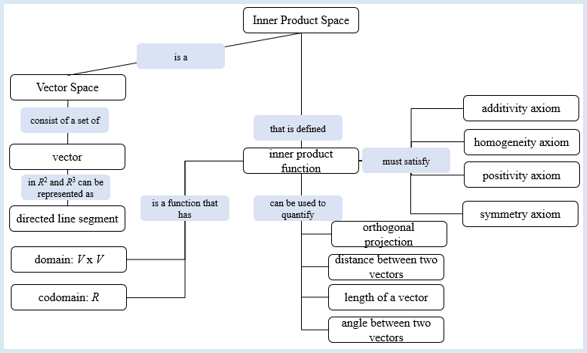
\includegraphics[width=100mm]{images/expert_map.png}
        \end{center}
        \caption{Criterion map developed by the class teacher}
    \end{figure}
\end{frame}

\begin{frame}{Expert evaluation on the students' generated map:cont'd}
    \begin{itemize}
        \item The teacher had developed a \textcolor{blue}{criterion map} beforehand.
        \item After the experiment, she created a \textcolor{blue}{grading rubric} accordingly, based on the \textcolor{blue}{completeness} of information in the student’s map and its \textcolor{blue}{accuracy}. 
        \item An information could be conveyed by different propositions with respect to the criterion map, but variation were limited since the subject was Mathematics.
    \end{itemize}
\end{frame}

\begin{frame}{Survey on learners' peceptions toward the activities}
    \begin{itemize}
        \item <1-3>The survey consists of 15 \textcolor{blue}{close-ended} items \& 6 \textcolor{blue}{open-ended} items. 
        
        \item <1>The closed-ended items were adopted from the User Experience Questionnaire, an Indonesian version \cite{Santoso2016MeasuringEnvironment}
        
        \item <2>It covers the \textcolor{blue}{perspectives of the students on the task itself} (e.g., attractiveness and stimulation scales) and \textcolor{blue}{the system used} (or non-task; e.g., perspicuity scale). 
        
        \item <3>The six open-ended questions were given to uncover the \textcolor{blue}{positive and negative experiences} of the students during the experiment.
    \end{itemize}
    
\end{frame}
\begin{frame}{Survey on learners' perceptions toward the activities (cont'd)}
    \begin{figure}[tb]
        \begin{center}
            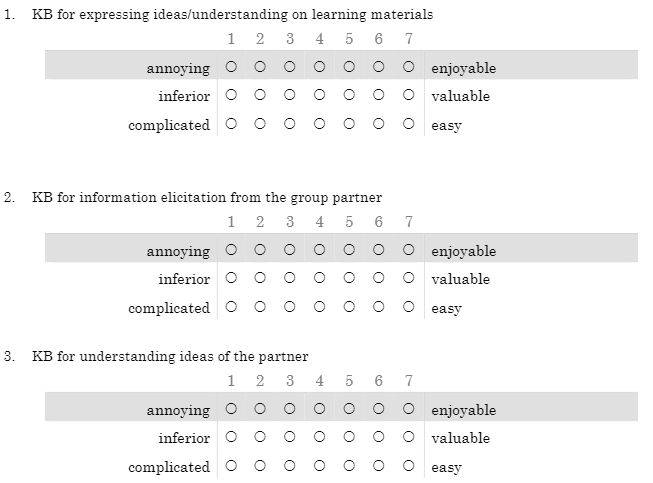
\includegraphics[width=70mm]{images/rqa_questionnaire_closed.png}
        \end{center}
        \caption{Closed-ended items}
        \label{questionnaire_close}
    \end{figure}
\end{frame}
\begin{frame}{Survey on learners' perceptions toward the activities (cont'd)}
    \begin{figure}[tb]
        \begin{center}
            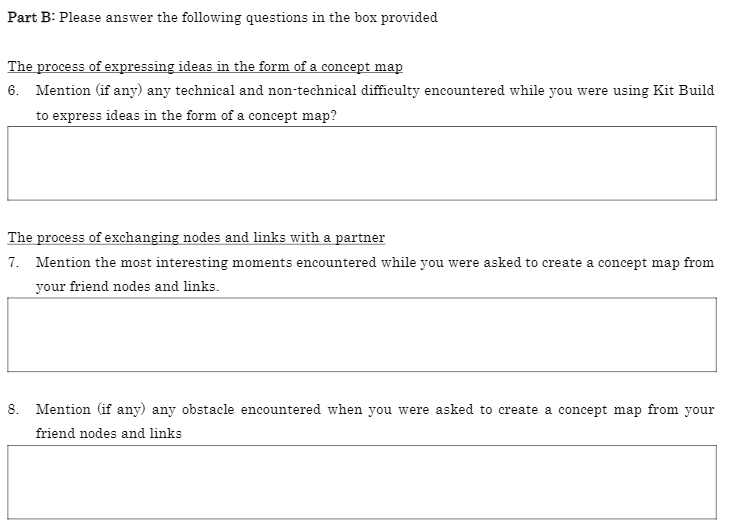
\includegraphics[width=70mm]{images/rqa_questionnaire_open.png}
        \end{center}
        \caption{Open-ended items}
        \label{questionnaire_open}
    \end{figure}
\end{frame}

\subsection{Results \& discussions}
\begin{frame}{Results (1): Overall group performances}
\begin{table}[tb]
    \caption{Descriptive statistics}
    \label{a1::group_performance}
    \begin{center}
        \begin{tabular}{c|c|c}
            \hline
            & Individual-map score & Group-map score\\
            \hline
            $M$ & 72.21 & 90 \\
            $SD$ & 18.22 & 7.31 \\
            $Min.$ & 41.43 & 75.71 \\
            $Max.$ & 98.57 & 100 \\
            \hline
        \end{tabular}
       
    \end{center}
    
    {\footnotesize
    \begin{itemize}
        \item A paired-samples t-test is conducted to compare the group average individual score and the group map score.
        \item The results of the \textcolor{blue}{group maps} ($M = 90, SD = 7.31$) showed \textcolor{teal}{increasing scores} compared to individual maps ($M = 72.21, SD = 18.22), t(20) = 4.92, p < .01$).
        \item The observed standardized \textcolor{teal}{effect size was large} (Cohen’s $d = .87$). 
    \end{itemize}
    }
    
\end{table}


\end{frame}

\begin{frame}{Results (1): Scores from the average of individual and group maps, along with the differences between the two scores}

\begin{figure}[tb]
    \begin{center}
        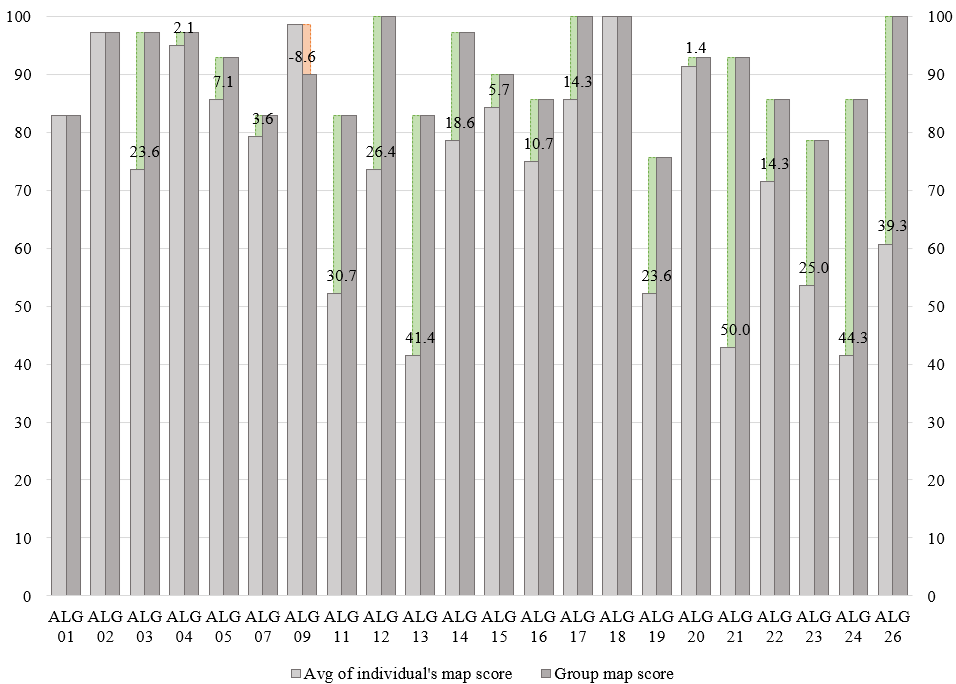
\includegraphics[width=70mm]{images/rqa_map_score_distribution.png}
    \end{center}
    \caption{Almost all groups produce high-quality collaborative products.}
    \label{a1::mapscore_distribution}
\end{figure}

\begin{block}{}
    Almost all groups produce high-quality collaborative products.
\end{block}

\end{frame}

\begin{frame}{Results (1): Distribution of correctness level in all individual and group propositions}
\begin{table}[tb]
    %\caption{Distribution of correctness level in all individual and group propositions}
    \label{dist_correct}
    \begin{center}
        \begin{tabular}{ p{5cm}|p{2cm}|p{2cm}  }
            \hline
            Level of correctness & Individual-map (\%) & Group-map (\%)\\
            \hline
            The true proposition & 64 & 81 \\
            The false proposition with a minor error & 5 & 7 \\
            The false proposition with a moderate error & 10 & 7 \\
            The false proposition with a fatal error & 21 & 5 \\
            \hline
        \end{tabular}
    \end{center}
\end{table}
\end{frame}

\begin{frame}{Research focus}

\textcolor{blue}{Aim}:
    To identify the effect of the RKB approach on collaborative concept mapping in a practical classroom
    
\begin{block}{Sub-research questions}
    \begin{enumerate}
        \item Whether or not students are able to produce high quality group products? If so, to what extent?
        \item \textcolor{blue}{How is the perceptions of the students while following the activities?}
\end{enumerate}
\end{block}

\end{frame}

\begin{frame}{Results (2): Questionnaire results: closed-ended items}
    \begin{figure}[tb]
    \begin{center}
        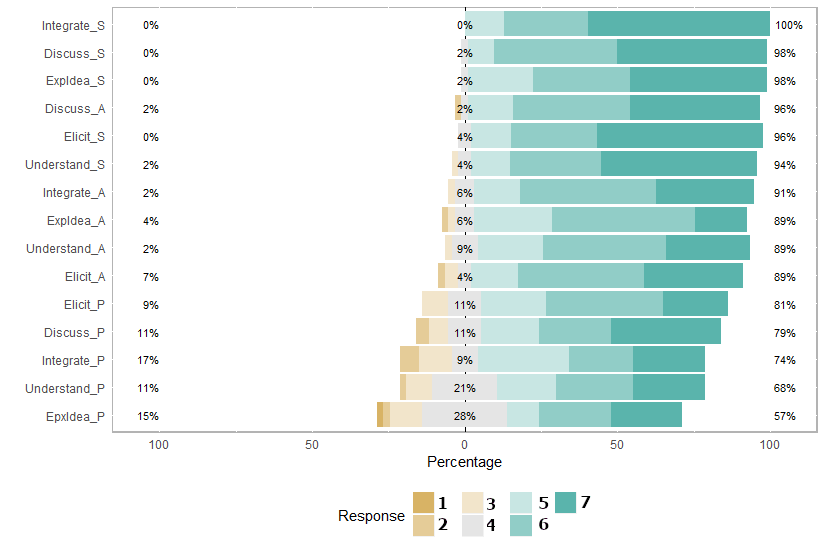
\includegraphics[width=85mm]{images/rqa_questionnaire_response.png}
    \end{center}
    \caption{Overall, the activity was \textcolor{teal}{valuable rather than inferior} (stimulation scale), and \textcolor{teal}{enjoyable rather than annoying} (attractiveness scale).}  
    % Though the items related to perspicuity (complicated vs. easy) had the lowest ranks among others, the mean scores of those items were above 5.00.
    \end{figure}
\end{frame}

\begin{frame}{Results (2): Questionnaire results: open-ended items}
\begin{itemize}
    \item <1> 60\% agreed that the \textcolor{teal}{most attractive phase} was the phase when they could \textcolor{teal}{see the difference} between the initial concept map and the reconstructed map (e.g., "I was glad to see the different way to connect the nodes by my friend").
    \item <2> The KB visualization of difference map also helped them to \textcolor{teal}{realize their mistakes} (14.9\%, e.g., "I realized if I have misconceptions or incorrect notions") and made them \textcolor{teal}{understand  their partner} (8.9\%, e.g., "I need to guess and try to understand perspectives of my friend's concept map.")
    \item <3> The KB links aided students in \textcolor{teal}{detecting alternatives perspectives} as well (25.5\%, e.g., "It is interesting to see the variety of my friends’ concepts and discussing it together.")
    \item <4> Students faced \textcolor{purple}{difficulties in integrating different perspectives} (15\%), especially when they had many differences (6.4\%).
\end{itemize}
\end{frame}
\begin{frame}{Key finding}
\textcolor{blue}{Research aim [A]}: To identify the effectiveness of the RKB approach for collaborative concept mapping in a practical classroom
\begin{block}{}
    \begin{enumerate}
        \item The students tend to build \textcolor{teal}{high-quality group products}. 
        \item The students perceive \textcolor{teal}{positive responses} toward the activities.  
    \end{enumerate}
   
\end{block}

\end{frame}

% The perceptions of the students revealed that the KB was valuable for integrating ideas in a group, eliciting information from the partner, and discussing differences in ideas.Consistently,  these three activities were getting the highest scores on the attractiveness scale.  The students also found that discussion and integration were the most complicated parts, along with understanding the comprehension of their partners.

\begin{frame}{Research objectives: Revisit}
    Based on the challenges mentioned above, we define the main purposes of this study are as follow: 
    \begin{enumerate}[A]
        \item \textcolor{lightgray}{to identify the effectiveness of the RKB approach for collaborative concept mapping in a practical classroom;}
        %\begin{enumerate}
        %    \item \textcolor{blue}{Collaborative product evaluation
        %    \item Exploring students' perceptions toward the activity}
        %\end{enumerate}
        
        \item \textcolor{blue}{to investigate how individual differences in prior knowledge has potentially influenced collaborative-learning effectiveness and the students' perceptions toward the activities;} 
        \begin{enumerate}[3]
            \item \textcolor{blue}{Analyzing the effect of different group formation on collaboration}
        \end{enumerate}
        
        \item to analyze how similarity of individual knowledge and comprehension  of partner's representation could predict the final collaborative products.
        %\begin{enumerate}[4]
        %    \item Predicting group outcomes based on individual maps
        %\end{enumerate}
    \end{enumerate} 
\end{frame}

